% ============================================================
\section{Actividad 1: Evaluación de estimadores}
% ============================================================

Se evalúan las propiedades estadísticas de los estimadores Varianza--Tiempo
(\texttt{vt2}) y Log--Escala (\texttt{LD2}) sobre secuencias discretas
independientes e idénticamente distribuidas. El valor teórico de referencia
es $H_0 = 0.5$.

% ------------------------------------------------------------
\subsection{Prueba de Sesgo}
% ------------------------------------------------------------

Se evaluó el sesgo bajo dos escenarios: muestra pequeña ($n = 1\,000$) y
muestra grande ($n = 100\,000$), con $10\,000$ realizaciones
$\mathcal{N}(0,1)$ en cada caso. Los parámetros de ajuste normal obtenidos
con \texttt{normfit} se consolidan en la Tabla~\ref{tab:sesgo}.

\begin{table}[H]
\centering
\caption{Parámetros de ajuste normal (\texttt{normfit}) para la prueba de sesgo.}
\label{tab:sesgo}
\renewcommand{\arraystretch}{1.3}
\begin{tabular}{rcccc}
\toprule
$n$ & $\hat{\mu}_{\text{VT}}$ & $\hat{\sigma}_{\text{VT}}$
    & $\hat{\mu}_{\text{LD}}$ & $\hat{\sigma}_{\text{LD}}$ \\
\midrule
$1\,000$   & $0.4967$ & $0.0289$ & $0.4982$ & $0.0347$ \\
$100\,000$ & $0.4996$ & $0.0099$ & $0.4999$ & $0.0063$ \\
\bottomrule
\end{tabular}
\end{table}

\begin{figure}[H]
    \centering
    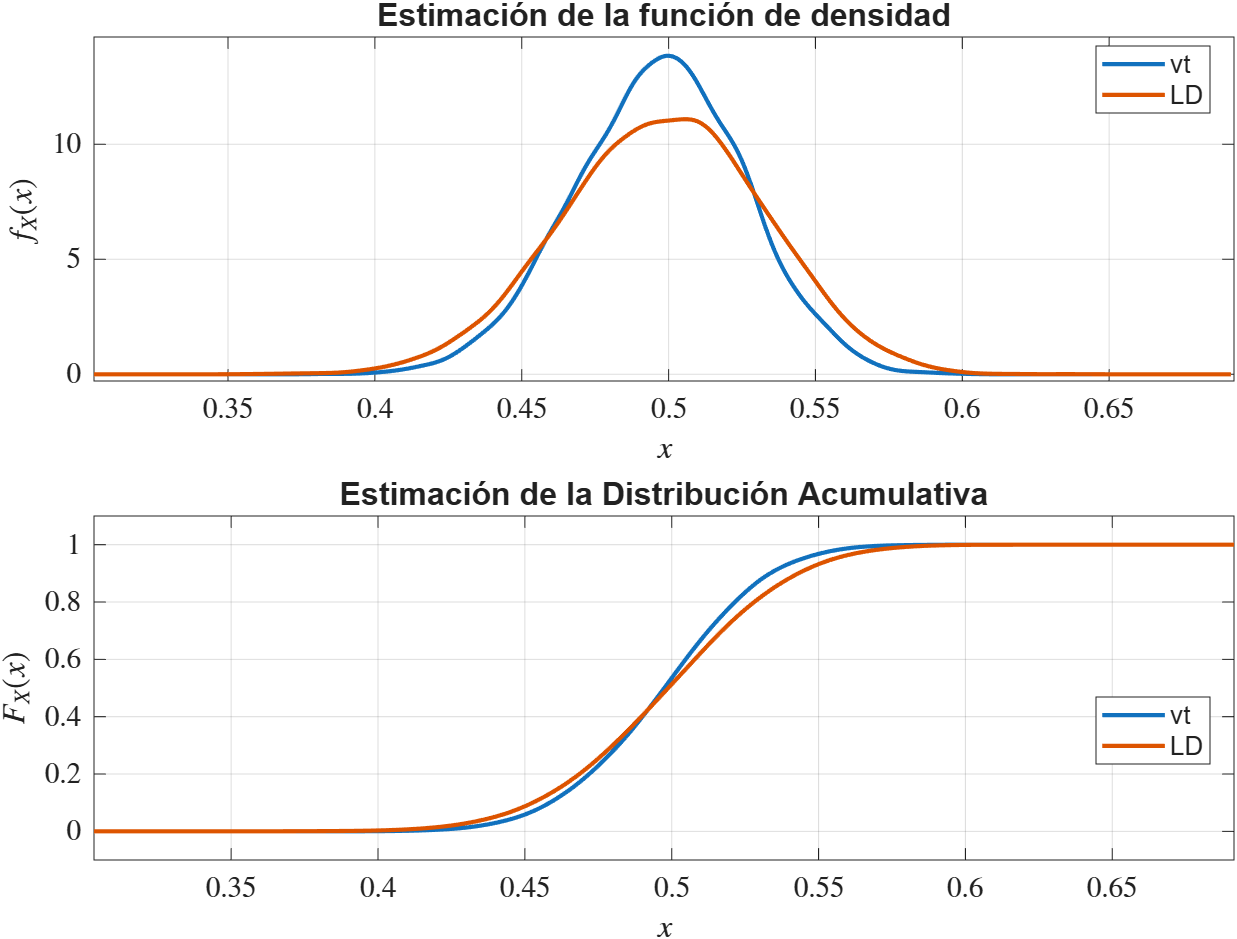
\includegraphics[width=0.88\textwidth]{actividades/actividad1/imgs/sesgo_muestra_1000.png}
    \caption{PDF y CDF empíricas de $\hat{H}$ para VT y LD
             ($n = 1\,000$, $10\,000$ repeticiones, $\mathcal{N}(0,1)$).}
    \label{fig:sesgo_1000}
\end{figure}

\begin{figure}[H]
    \centering
    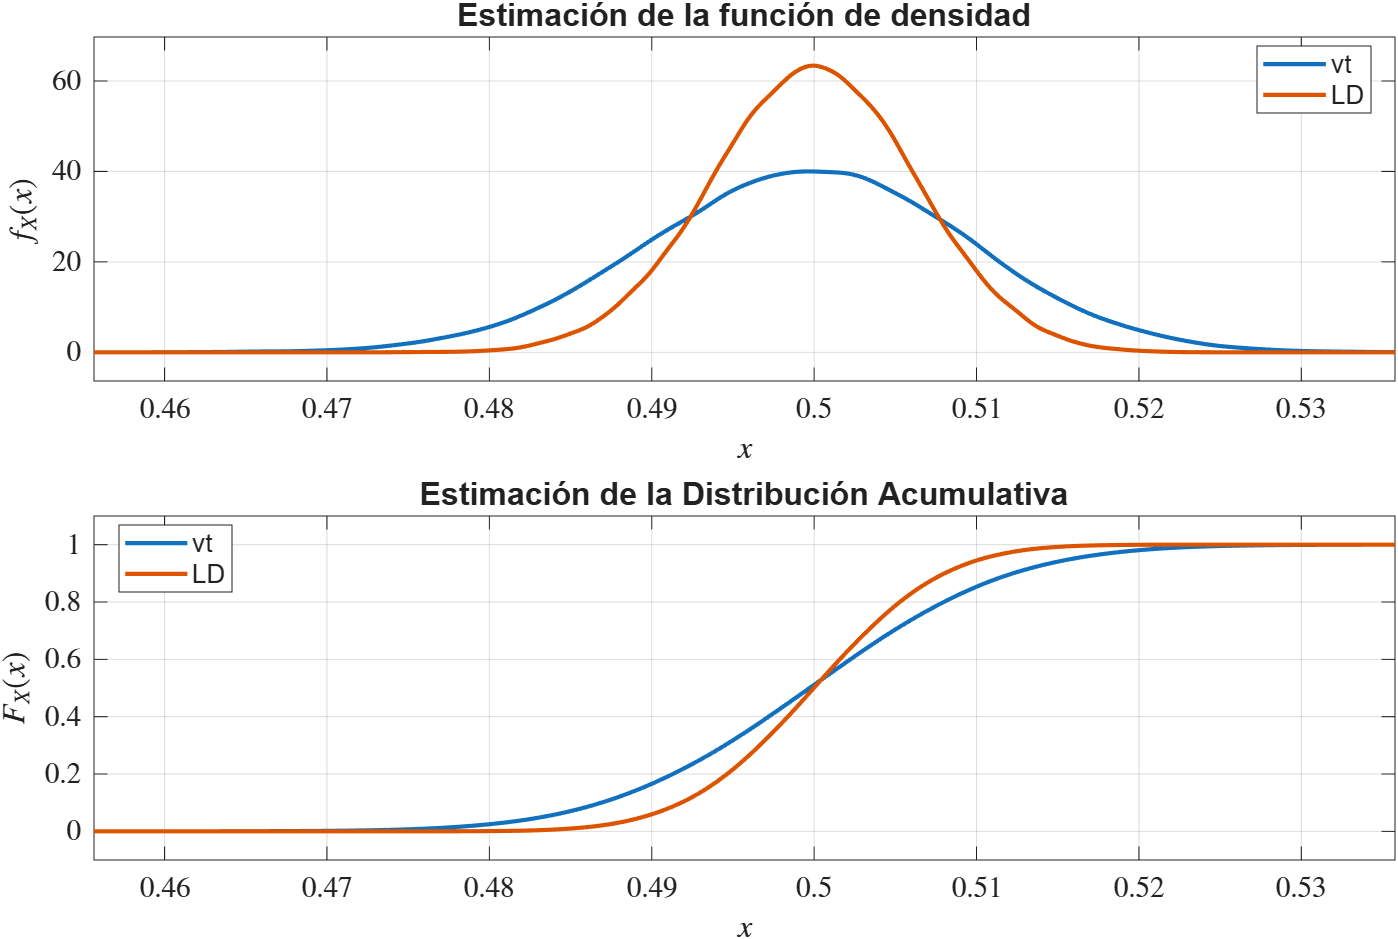
\includegraphics[width=0.88\textwidth]{actividades/actividad1/imgs/sesgo_muestra_100000.png}
    \caption{PDF y CDF empíricas de $\hat{H}$ para VT y LD
             ($n = 100\,000$, $10\,000$ repeticiones, $\mathcal{N}(0,1)$).}
    \label{fig:sesgo_100000}
\end{figure}

\begin{figure}[H]
    \centering
    \begin{subfigure}[b]{0.48\textwidth}
        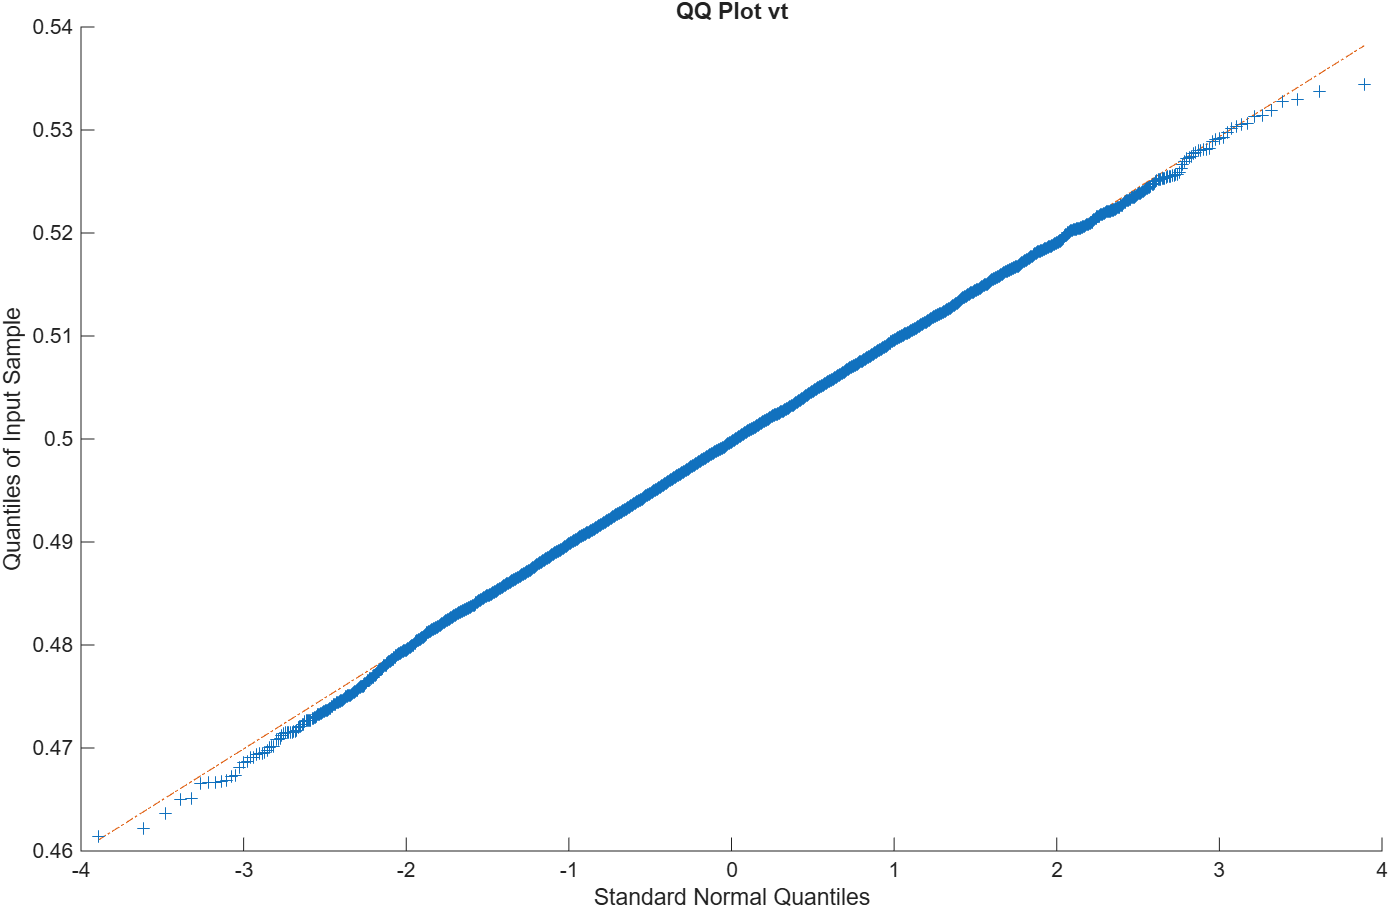
\includegraphics[width=\textwidth]{actividades/actividad1/imgs/qqplot_muestra_vt.png}
        \caption{QQ-plot estimador VT ($n = 100\,000$).}
    \end{subfigure}
    \hfill
    \begin{subfigure}[b]{0.48\textwidth}
        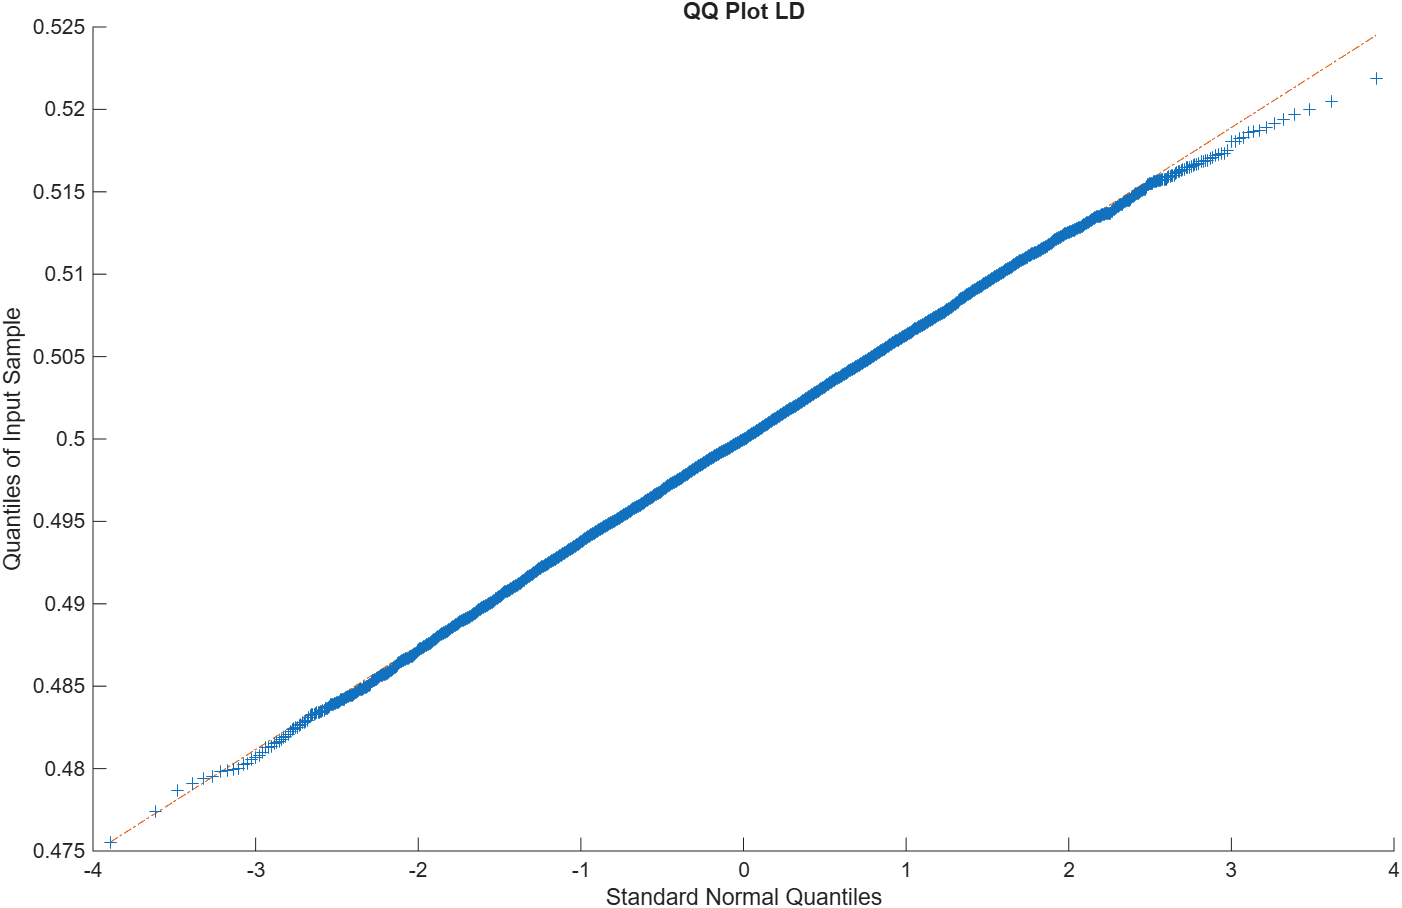
\includegraphics[width=\textwidth]{actividades/actividad1/imgs/qqplot_muestra_ld.png}
        \caption{QQ-plot estimador LD ($n = 100\,000$).}
    \end{subfigure}
    \caption{La alineación con la recta de referencia confirma distribución
             normal en ambos estimadores, justificando el uso de \texttt{normfit}.}
    \label{fig:qqplots}
\end{figure}

Para $n = 1\,000$ (Figura~\ref{fig:sesgo_1000}), ambos estimadores muestran
sesgo despreciable ($-0.0033$ para VT y $-0.0018$ para LD), pero las
distribuciones son notablemente anchas. En este régimen VT es ligeramente
más eficiente: su desviación estándar ($0.0289$) es un 17\,\% menor que la
de LD ($0.0347$), es decir, para muestras pequeñas LD no ofrece ventaja en
varianza.

Para $n = 100\,000$ (Figura~\ref{fig:sesgo_100000}), la situación se invierte:
ambas distribuciones se concentran fuertemente en $H_0 = 0.5$ y el sesgo
permanece negligible, pero ahora LD presenta una desviación estándar un
36\,\% menor que VT ($0.0063$ vs.\ $0.0099$). Esta inversión queda también
reflejada en los QQ-plots (Figura~\ref{fig:qqplots}): VT exhibe una leve
desviación en las colas, mientras que LD se ajusta con mayor fidelidad a la
recta de referencia para muestras grandes.

% ------------------------------------------------------------
\subsection{Prueba de Consistencia}
% ------------------------------------------------------------

Se evaluó la convergencia de cada estimador al aumentar el tamaño de muestra.
Se generaron $1\,000$ realizaciones para cada $N \in \{2^{14},\,2^{16},\,
2^{18},\,2^{20}\}$ con distribución $\mathcal{N}(0,1)$.

\begin{figure}[H]
    \centering
    \begin{subfigure}[b]{0.88\textwidth}
        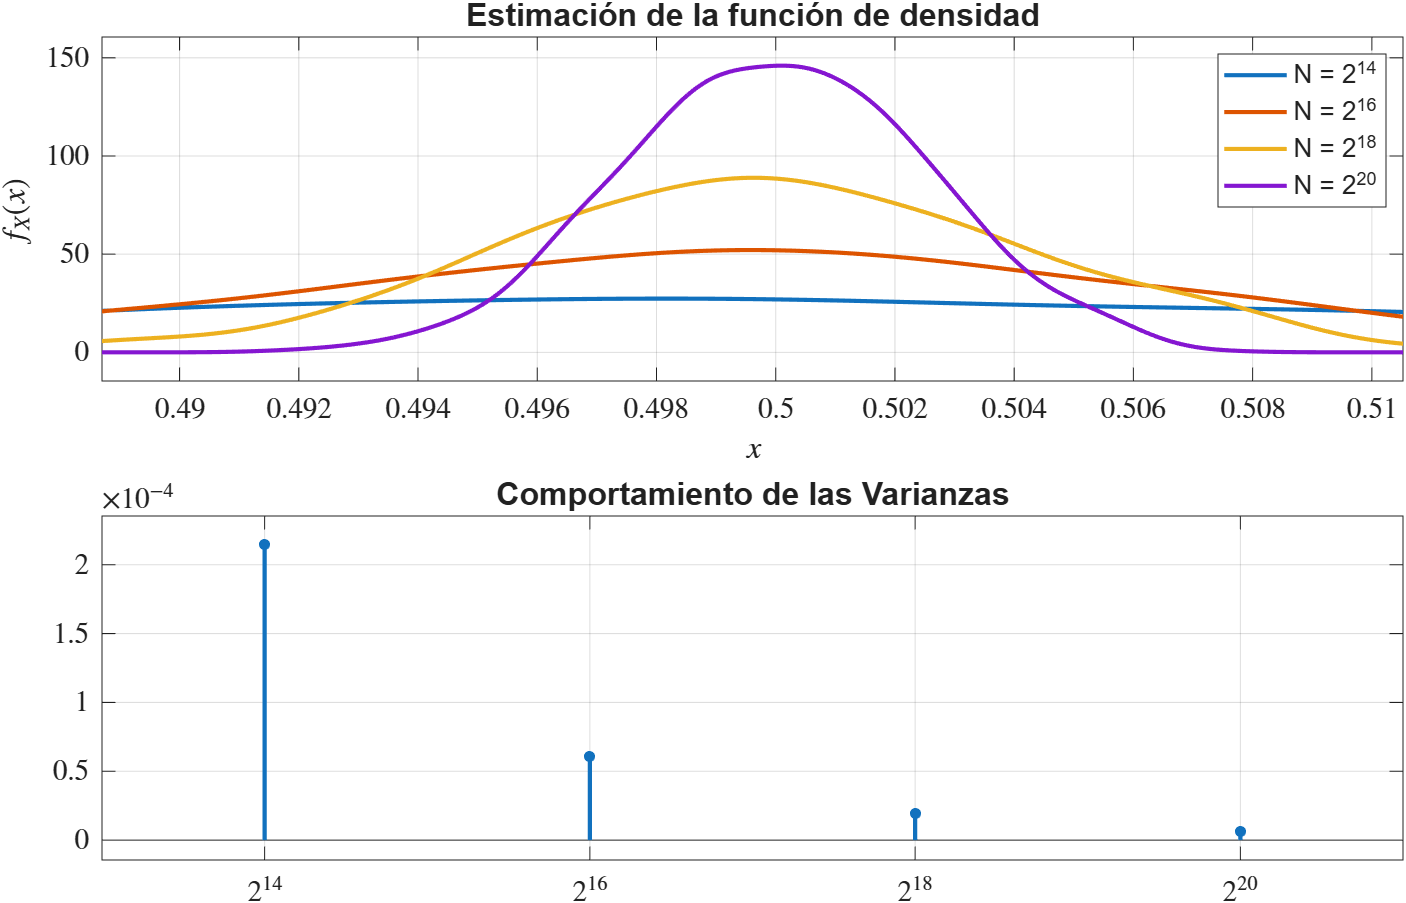
\includegraphics[width=\textwidth]{actividades/actividad1/imgs/consistencia_ld.png}
        \caption{Estimador LD: la PDF se estrecha progresivamente y la
                 varianza cae de $2.13\times10^{-4}$ ($N=2^{14}$) a
                 $6.7\times10^{-5}$ ($N=2^{20}$).}
    \end{subfigure}
    \vspace{0.4em}
    \begin{subfigure}[b]{0.88\textwidth}
        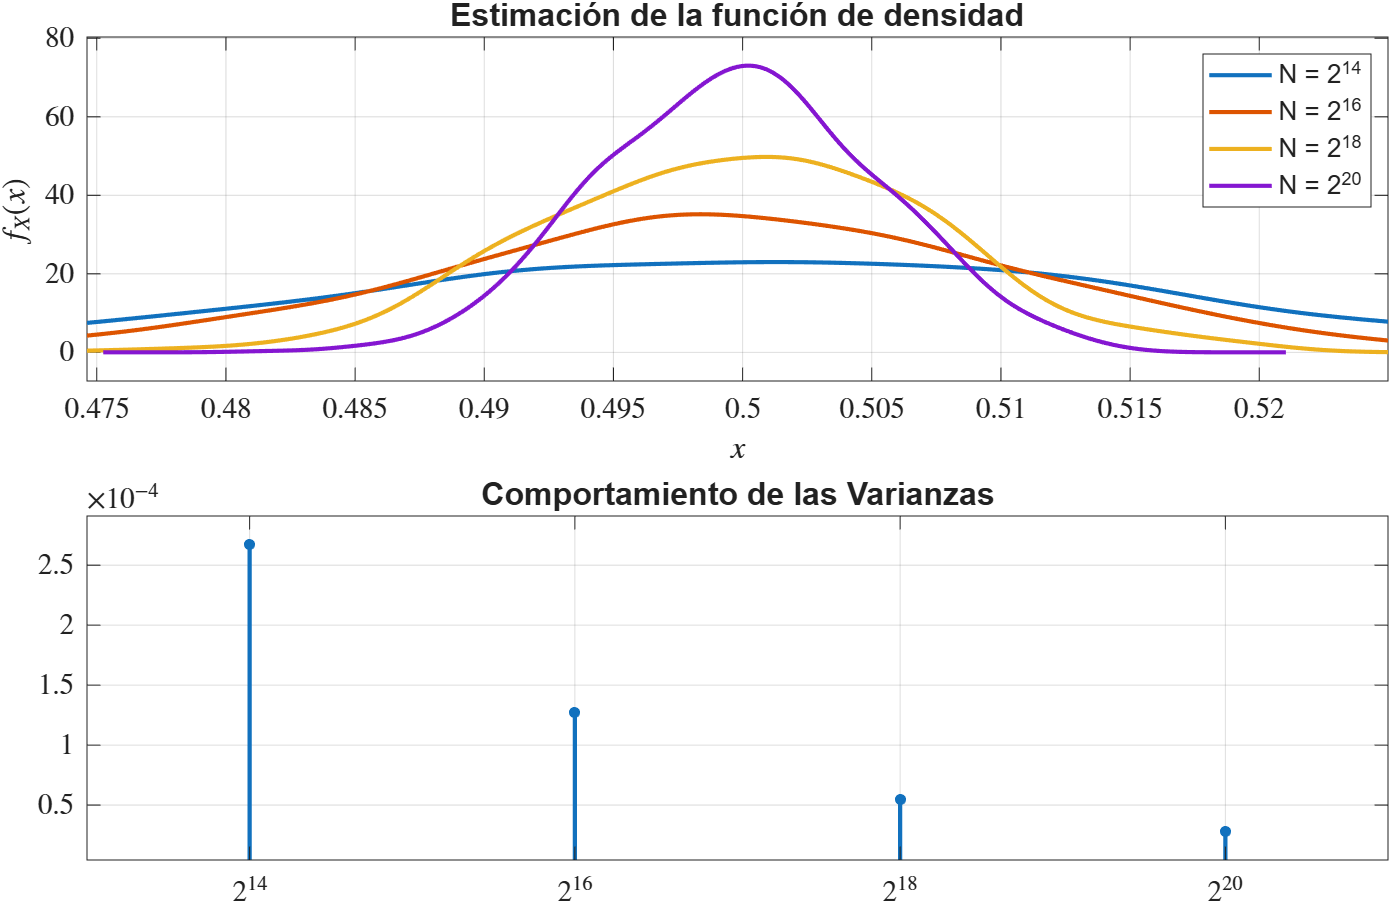
\includegraphics[width=\textwidth]{actividades/actividad1/imgs/consistencia_vt.png}
        \caption{Estimador VT: convergencia más lenta; la varianza cae de
                 $2.65\times10^{-4}$ ($N=2^{14}$) a $2.7\times10^{-4}$
                 ($N=2^{20}$).}
    \end{subfigure}
    \caption{Consistencia de los estimadores VT y LD. Las PDFs se concentran
             en $H_0 = 0.5$ al crecer $N$, y las varianzas disminuyen
             monotónicamente (panel inferior de cada subfigura).}
    \label{fig:consistencia}
\end{figure}

Ambos estimadores son consistentes: las densidades se estrechan y centran en
$H_0 = 0.5$ al aumentar $N$, y las varianzas decrecen monótonamente.
LD converge más rápido: para $N = 2^{20}$ su varianza es
$\approx 6.7\times10^{-5}$, frente a $\approx 2.7\times10^{-4}$ de VT,
una reducción cuatro veces mayor.

% ------------------------------------------------------------
\subsection{Prueba de Eficiencia}
% ------------------------------------------------------------

La eficiencia se mide comparando la varianza de cada estimador para un mismo
tamaño de muestra $n$. Se usaron $1\,000$ repeticiones para cada
$n \in \{1000,\,2000,\,5000,\,10000,\,\allowbreak20000,\,50000,\,100000\}$.

\begin{figure}[H]
    \centering
    \begin{subfigure}[b]{0.88\textwidth}
        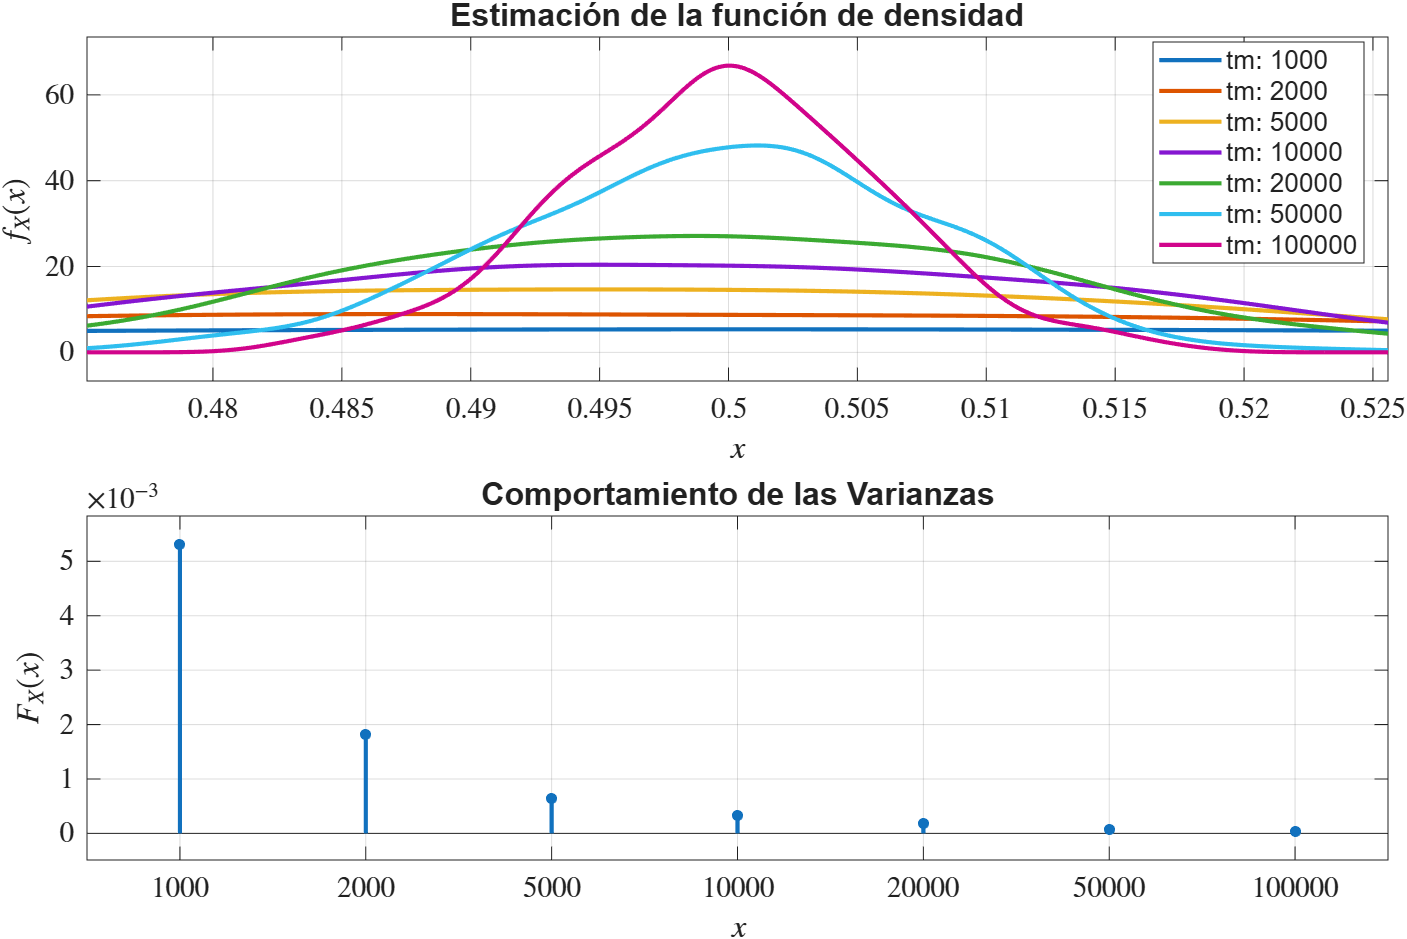
\includegraphics[width=\textwidth]{actividades/actividad1/imgs/eficiencia_ld.png}
        \caption{Estimador LD.}
    \end{subfigure}
    \vspace{0.4em}
    \begin{subfigure}[b]{0.88\textwidth}
        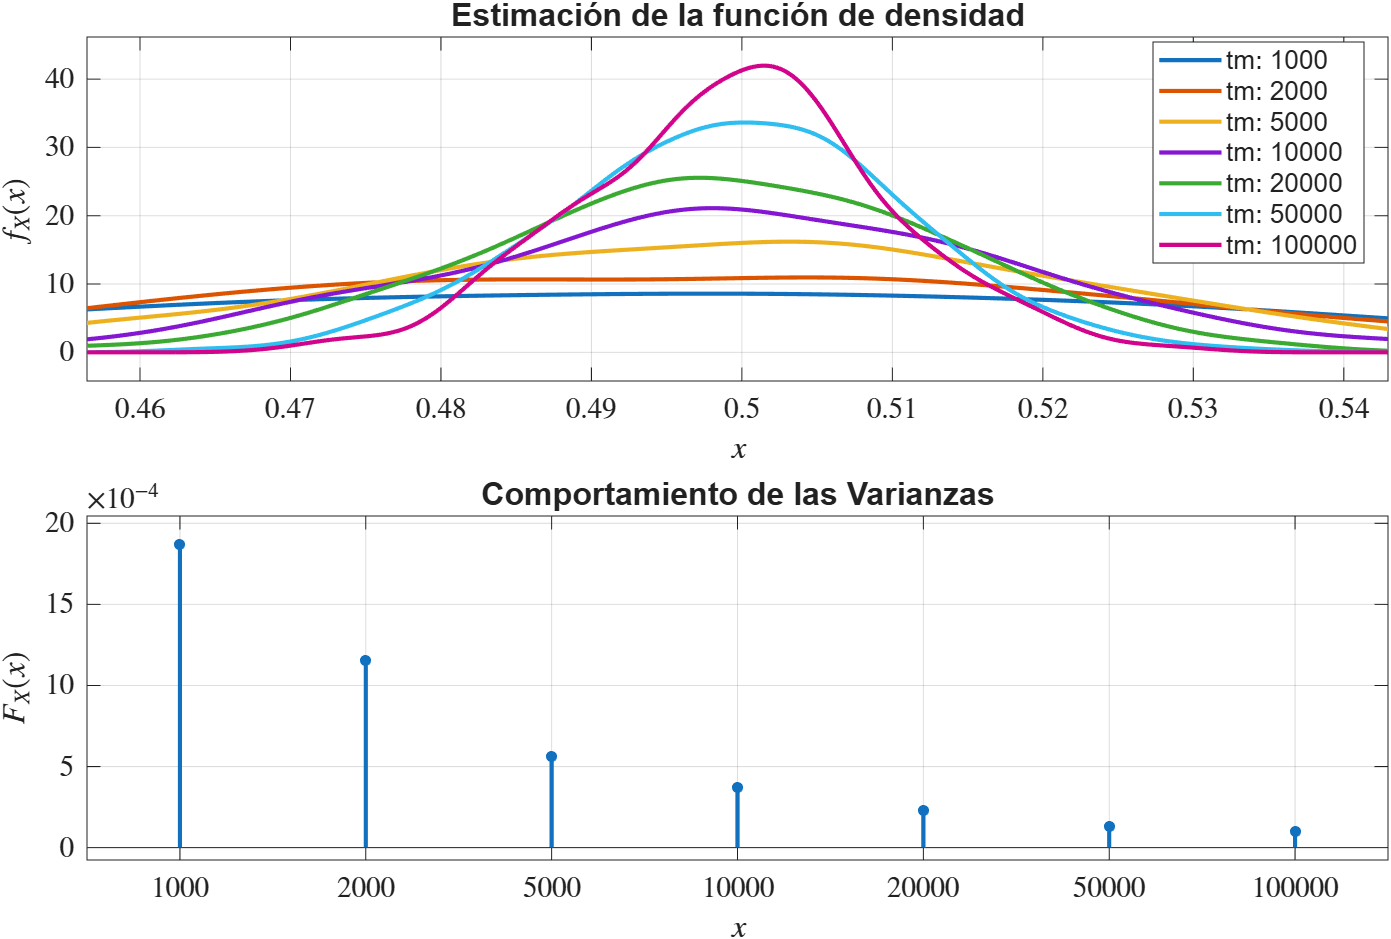
\includegraphics[width=\textwidth]{actividades/actividad1/imgs/eficiencia_vt.png}
        \caption{Estimador VT.}
    \end{subfigure}
    \caption{PDF empírica y comportamiento de las varianzas de VT y LD
             para distintos tamaños de muestra $n$.}
    \label{fig:eficiencia}
\end{figure}

La Tabla~\ref{tab:varianzas} consolida las varianzas obtenidas. Para $n \leq 2\,000$,
VT resulta más eficiente; a partir de $n = 5\,000$ LD supera a VT, y a
$n = 100\,000$ su varianza es $\approx 2.65$ veces menor.

\begin{table}[H]
\centering
\caption{Varianza de $\hat{H}$ en función del tamaño de muestra $n$.}
\label{tab:varianzas}
\renewcommand{\arraystretch}{1.3}
\begin{tabular}{rcc}
\toprule
$n$ & $\text{Var}(\hat{H}_{\text{VT}})$ & $\text{Var}(\hat{H}_{\text{LD}})$ \\
\midrule
$1\,000$   & $1.87\times10^{-3}$ & $5.31\times10^{-3}$ \\
$2\,000$   & $1.16\times10^{-3}$ & $1.82\times10^{-3}$ \\
$5\,000$   & $5.59\times10^{-4}$ & $6.43\times10^{-4}$ \\
$10\,000$  & $3.71\times10^{-4}$ & $3.27\times10^{-4}$ \\
$20\,000$  & $2.28\times10^{-4}$ & $1.83\times10^{-4}$ \\
$50\,000$  & $1.32\times10^{-4}$ & $6.76\times10^{-5}$ \\
$100\,000$ & $1.00\times10^{-4}$ & $3.77\times10^{-5}$ \\
\bottomrule
\end{tabular}
\end{table}

% ------------------------------------------------------------
\subsection{Prueba de Robustez}
% ------------------------------------------------------------

Se evaluó la sensibilidad de cada estimador ante cambios en la distribución
de la secuencia de entrada, usando cuatro distribuciones: Normal
$\mathcal{N}(0,1)$, Uniforme $\mathcal{U}(0,1)$, Exponencial $\text{Exp}(1)$
y $\text{Beta}(2,5)$, con $n = 100\,000$ y $1\,000$ repeticiones.

\begin{figure}[H]
    \centering
    \begin{subfigure}[b]{0.88\textwidth}
        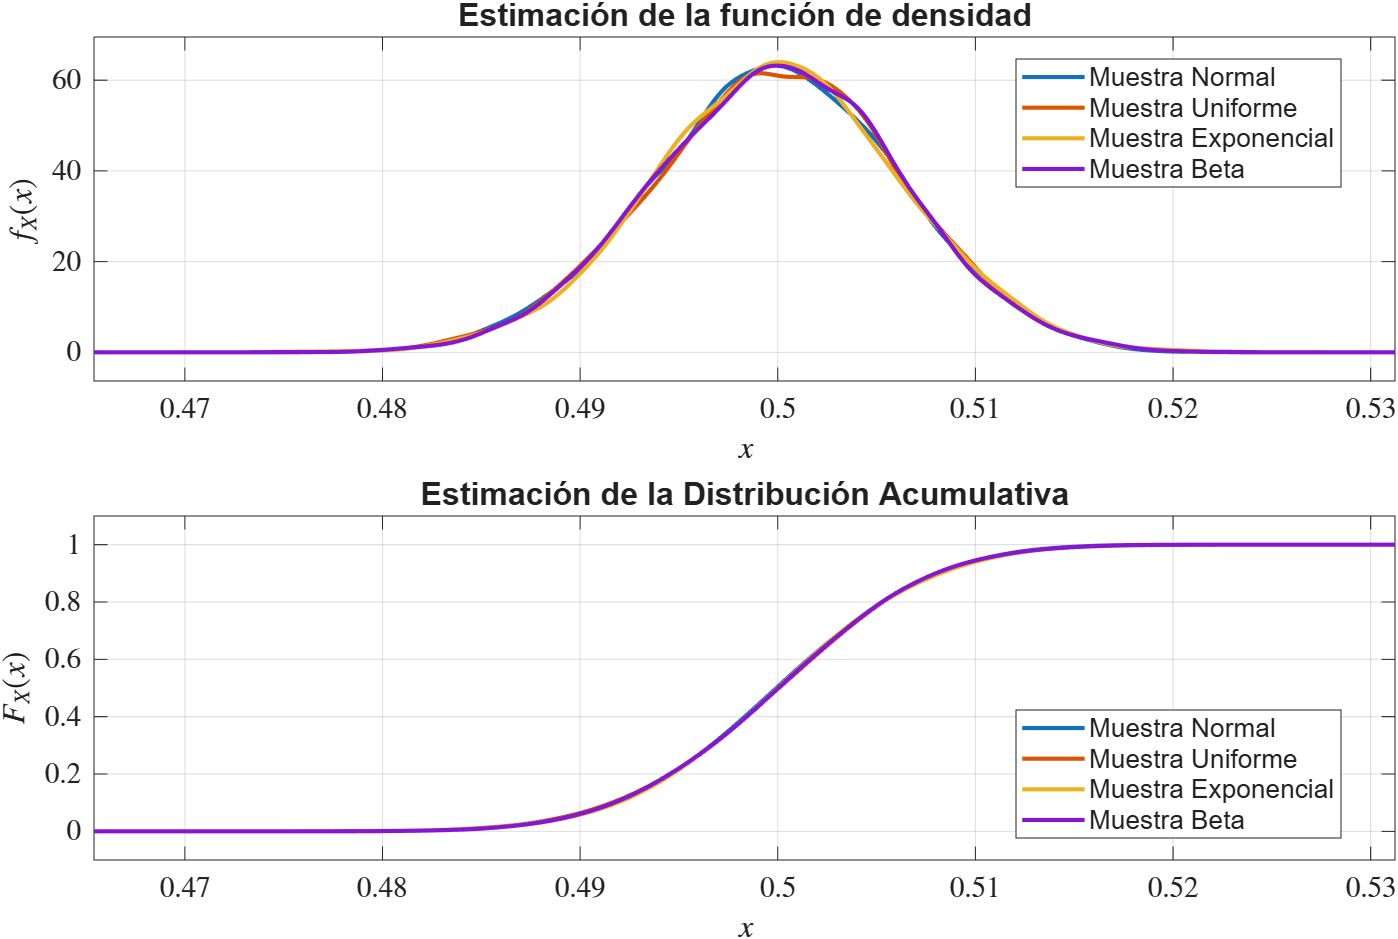
\includegraphics[width=\textwidth]{actividades/actividad1/imgs/robustes_ld.png}
        \caption{Estimador LD: las cuatro curvas son prácticamente
                 indistinguibles, con pico $\approx 63$.}
    \end{subfigure}
    \vspace{0.4em}
    \begin{subfigure}[b]{0.88\textwidth}
        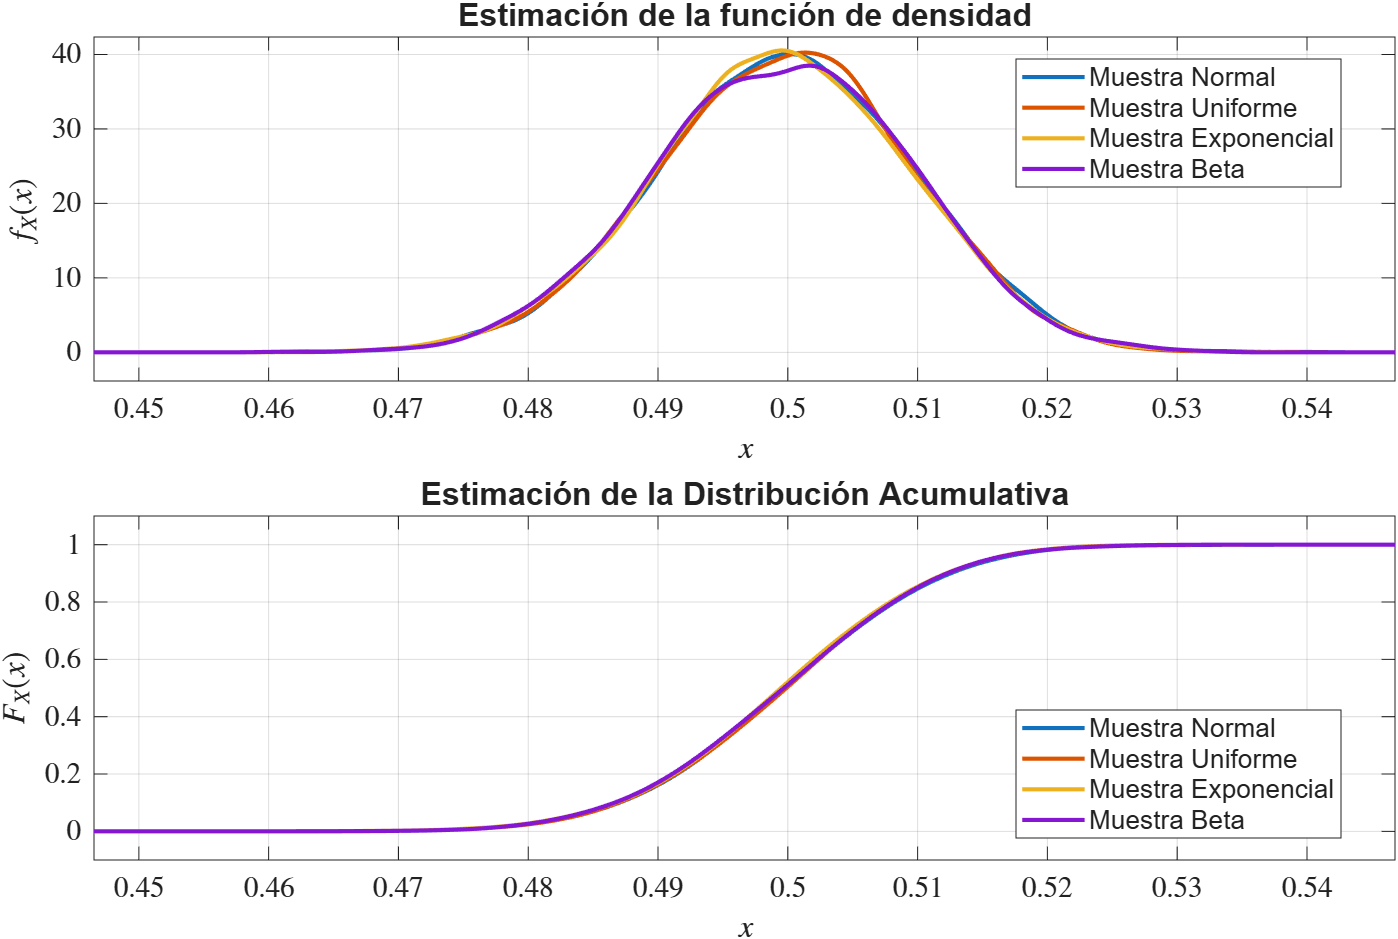
\includegraphics[width=\textwidth]{actividades/actividad1/imgs/robustes_vt.png}
        \caption{Estimador VT: las cuatro curvas también se superponen,
                 con pico $\approx 40$ y ligera separación entre distribuciones.}
    \end{subfigure}
    \caption{Robustez de los estimadores VT y LD ante distintas distribuciones
             de entrada ($n = 100\,000$, $1\,000$ repeticiones).}
    \label{fig:robustez}
\end{figure}

Ambos estimadores exhiben alta robustez: las PDF y CDF para las cuatro
distribuciones se superponen casi perfectamente en ambos casos, centradas en
$H_0 = 0.5$. LD presenta mayor concentración (pico $\approx 63$ vs.\
$\approx 40$ de VT), lo que refleja su menor varianza independientemente de
la distribución de entrada. Ninguno de los dos estimadores muestra
sensibilidad apreciable ante cambios distribucionales para muestras grandes.

% ------------------------------------------------------------
\subsection{Resumen de la Actividad 1}
% ------------------------------------------------------------

\begin{table}[H]
\centering
\caption{Comparación de estimadores VT y LD por propiedad evaluada.}
\label{tab:resumen}
\renewcommand{\arraystretch}{1.3}
\begin{tabular}{lccc}
\toprule
\textbf{Propiedad} & \textbf{VT} & \textbf{LD} & \textbf{Ganador} \\
\midrule
Sesgo ($n < 5\,000$)         & $\hat{\sigma} = 0.0289$ & $\hat{\sigma} = 0.0347$ & \textbf{VT} \\
Sesgo ($n \geq 5\,000$)      & $\hat{\sigma} = 0.0099$ & $\hat{\sigma} = 0.0063$ & \textbf{LD} \\
Consistencia                 & Converge, varianza mayor  & Converge más rápido     & \textbf{LD} \\
Eficiencia ($n < 5\,000$)    & $\text{Var}$ menor        & $\text{Var}$ mayor      & \textbf{VT} \\
Eficiencia ($n \geq 5\,000$) & $\text{Var}\approx1.00\times10^{-4}$ & $\text{Var}\approx3.77\times10^{-5}$ & \textbf{LD} \\
Robustez                     & Alta                      & Alta                    & \textbf{Empate} \\
\bottomrule
\end{tabular}
\end{table}

Para muestras grandes ($n \geq 5\,000$), LD supera a VT en sesgo,
consistencia y eficiencia. Para muestras pequeñas ($n < 5\,000$), VT es más
eficiente y presenta menor dispersión. Ambos estimadores son igualmente
robustos ante cambios en la distribución de entrada.